\documentclass{article}
\usepackage{graphicx}
\usepackage{amsmath}
\usepackage{amsfonts}
\usepackage{bookmark}
\usepackage{booktabs}
\usepackage{exercises}
\graphicspath{ {./images/5.3} }
\usepackage{indentfirst}
\usepackage{amsthm}
\usepackage{yhmath}
\usepackage{geometry}
\usepackage{placeins}
\usepackage{csquotes}
\usepackage{pgfplots}
\newcommand*{\oldneg}{\mathord{\sim}}
\newcommand\showdiv[1]{\overline{\smash{)}#1}}
\newcommand\Mydiv[1]{%
\smash{\raise.3ex\hbox{$\big)$}}\mkern-8mu
        \overline{\enspace\strut#1}}
\setlength{\tabcolsep}{5pt}
\theoremstyle{definition}
\newtheorem{definition}{Definition}

\setlength{\parindent}{.5in}
\setlength{\parskip}{12pt}
\renewcommand{\arraystretch}{2}
\geometry{margin=1in}
\newcommand{\?}{\stackrel{?}{=}}
\pgfplotsset{width=7cm,compat=1.18}\usepgfplotslibrary{statistics}

\title{5.3 Answers}
\begin{document}
\maketitle

\section*{1}
The graph of a rational function $f$ has no horizontal asymptote when the degree of the function's numerator is greater than the degree of its 
denominator.

\section*{2}
Suppose that $f(x)=\frac{p(x)}{q(x)}$ such that $p(x)$ and $q(x)$ are polynomials with no common factors other than $\pm 1$.
One can find the $x$-intercepts of $f$ by finding the real zero's of $p(x)$. The vertical asymptotes are the real zero's of 
$q(x)$.

\section*{3}
C

\section*{4}
A

\section*{5}
B

\section*{6}
A

\section*{7}
This graph has no $x$-intercepts. Because the solutions of $x^2-1=0$ are $\pm 1$, the vertical asymptotes of the graph are $x=\pm 1$.

\section*{9}
Because there are no real solutions to the equation $x^2+9=0$, this graph has no $x$-intercepts. 
Because $x^2-2x-15=(x-5)(x+3)$, the solutions to the equation $x^2-2x-15=0$ are $5$ and $-3$, meaning the graph of this function has the vertical asymptotes 
$y=5$ and $y=-3$.

\section*{12}
Because $2x^2-3x-20=(2x+5)(x-4)$, the solutions to the equation $2x^2-3x-20$ are $-\frac{5}{2}$ and $4$, meaning the graph of this function has the 
$x$-intercepts $-\frac{5}{2}$ and $4$. Because there are no real solutions to the equation $x^2+1=0$, the graph of this function has no vertical asymptotes.

\section*{13}
The error here is that the vertical asymptotes of $f(x)$ occur at the zero of the denominator, not the numerator. Thus, because the solutions of 
$x^2-8x+7$ are $7$ and $1$, the vertical asymptotes of $f(x)$ are $y=7$ and $y=1$.

\section*{14}
Because the degrees of the polynomials on the numerator and denominator are the same, the horizonatal asymptote is $\frac{4}{1}=4$. C

\section*{20}
Because the degree of the polynomial on the numerator is greater than the one on the denominator, we know that there is no horizontal asymptote. 
In addition, the $x$-intercept of this graph is $x=2$, as $2$ is the solution to $x^3-8$. The vertical asymptotes are $x=\pm\sqrt{6}$, as those are the solutions of the 
equation $6-x^2=0$.
\newline 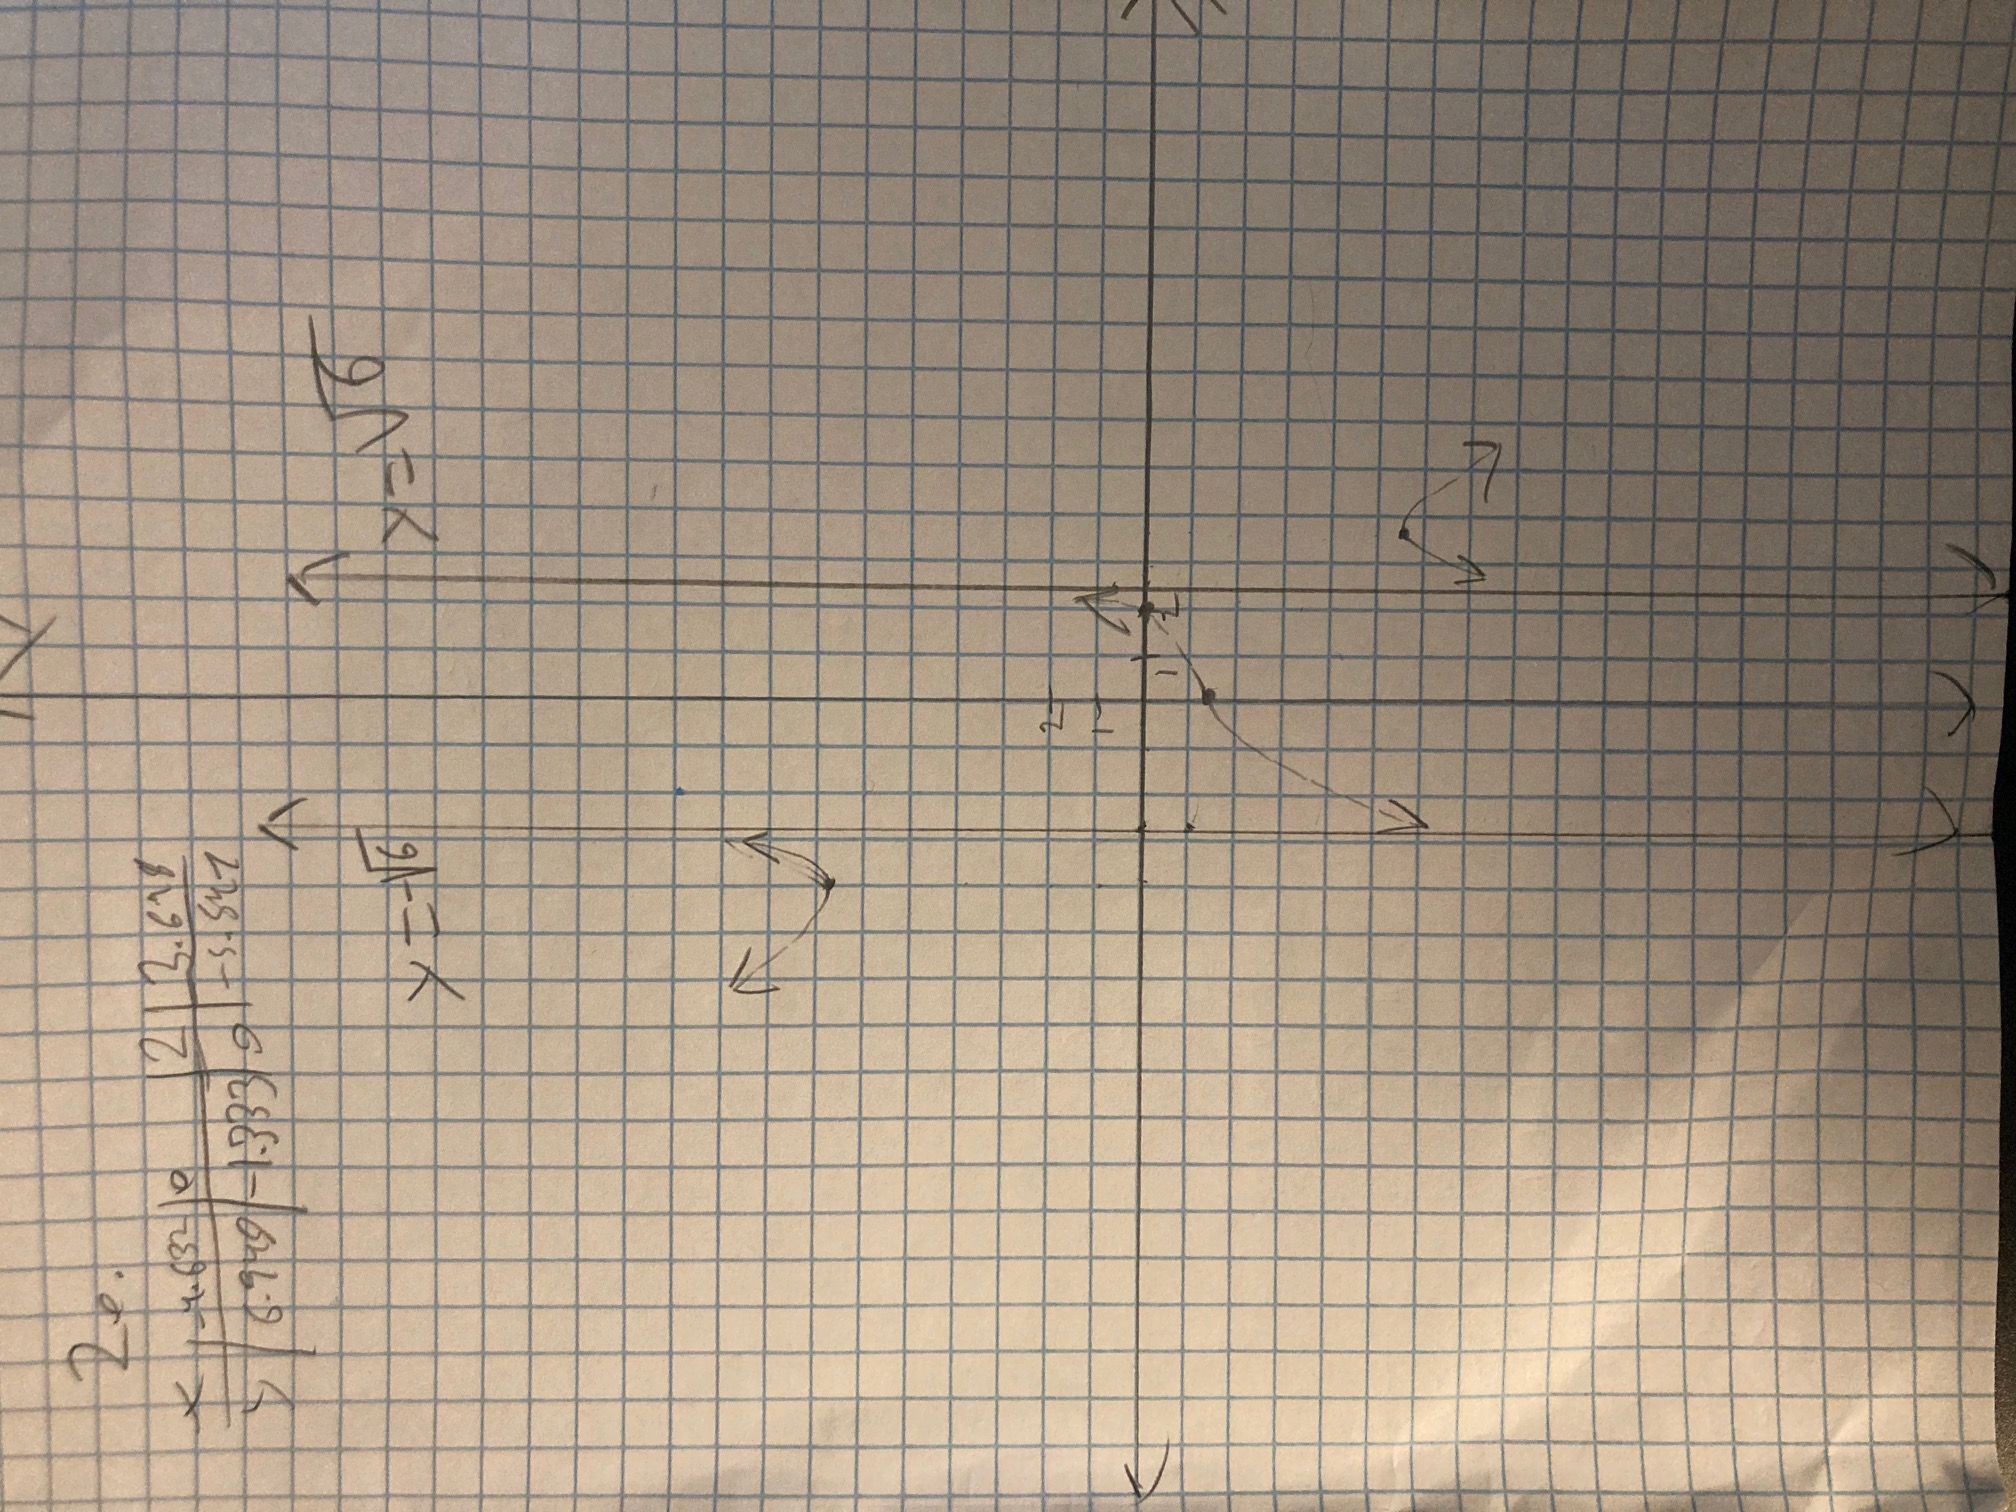
\includegraphics[width = 4in, height = 4in, angle = -90]{20}\newline

\section*{24}
Consider some rational function $f(x)=\frac{p(x)}{q(x)}$ where $p(x)$ and $q(x)$ are polynomials with no common factors other than $\pm 1$, 
and such that $m$ and $n$ are the degrees 
of $p(x)$ and $q(x)$, respectively. If $n<m$, we know that the graph's end behavior is the same as the graph of $y=\frac{a_m}{b_n}x^{m-n}$ where 
$a_m$ and $b_n$ are the leading coefficients of $p(x)$ and $q(x)$, respectively. Thus one example of a function whose graph has the same end behavior as the graph 
of $y=3x^2$ is $f(x)=\frac{9x^4+3}{3x^2}$. Another example is $f(x)=\frac{21x^6-3x+2}{7x^4}$.

\section*{28}
We know that $2=\frac{a}{0^2+b}$, meaning $a=2b$, and $1=\frac{a}{1^2+b}$. Thus
\[ 1=\frac{a}{1+b} \] \[ 1=\frac{2b}{1+b} \] \[ 2b=1+b \] \[ b=1 \] meaning $a=2(1)=2$.

\section*{30}
We know that $-1=\frac{a}{9+b}$, meaning $a=-9-b$, and $-6=\frac{a}{4+b}$. Thus
\[ -6=\frac{a}{4+b} \] \[ -6=\frac{-9-b}{4+b} \] \[ -24-6b=-9-b \] \[ -5b=15 \] \[ b=-3 \] meaning $a=-9+3=-6$.

\section*{36}
(a): We know that the volume of a cylinder is given by $V=\pi r^2h$. Now, we are also given that the tank must be built using $100$ cubic feet of concrete. Thus we can 
write $h$ in terms of $r$: \[ 100=\pi (r+1)^2(h+1) \] \[ 100=\pi (r^2+2r+1)(h+1) \] \[ h+1=\frac{100}{r^2\pi +2r\pi +\pi} \]
\[ h=\frac{100}{r^2\pi +2r\pi +\pi}-1 \]


(b): We know that the water the tank can hold is given by $\pi r^2h$. Thus we can use the equation for $h$ in part (a) to write:
\[ V=\pi r^2h=\pi r^2(\frac{100}{r^2\pi +2r\pi +\pi}-1) \] 


(c): \newline 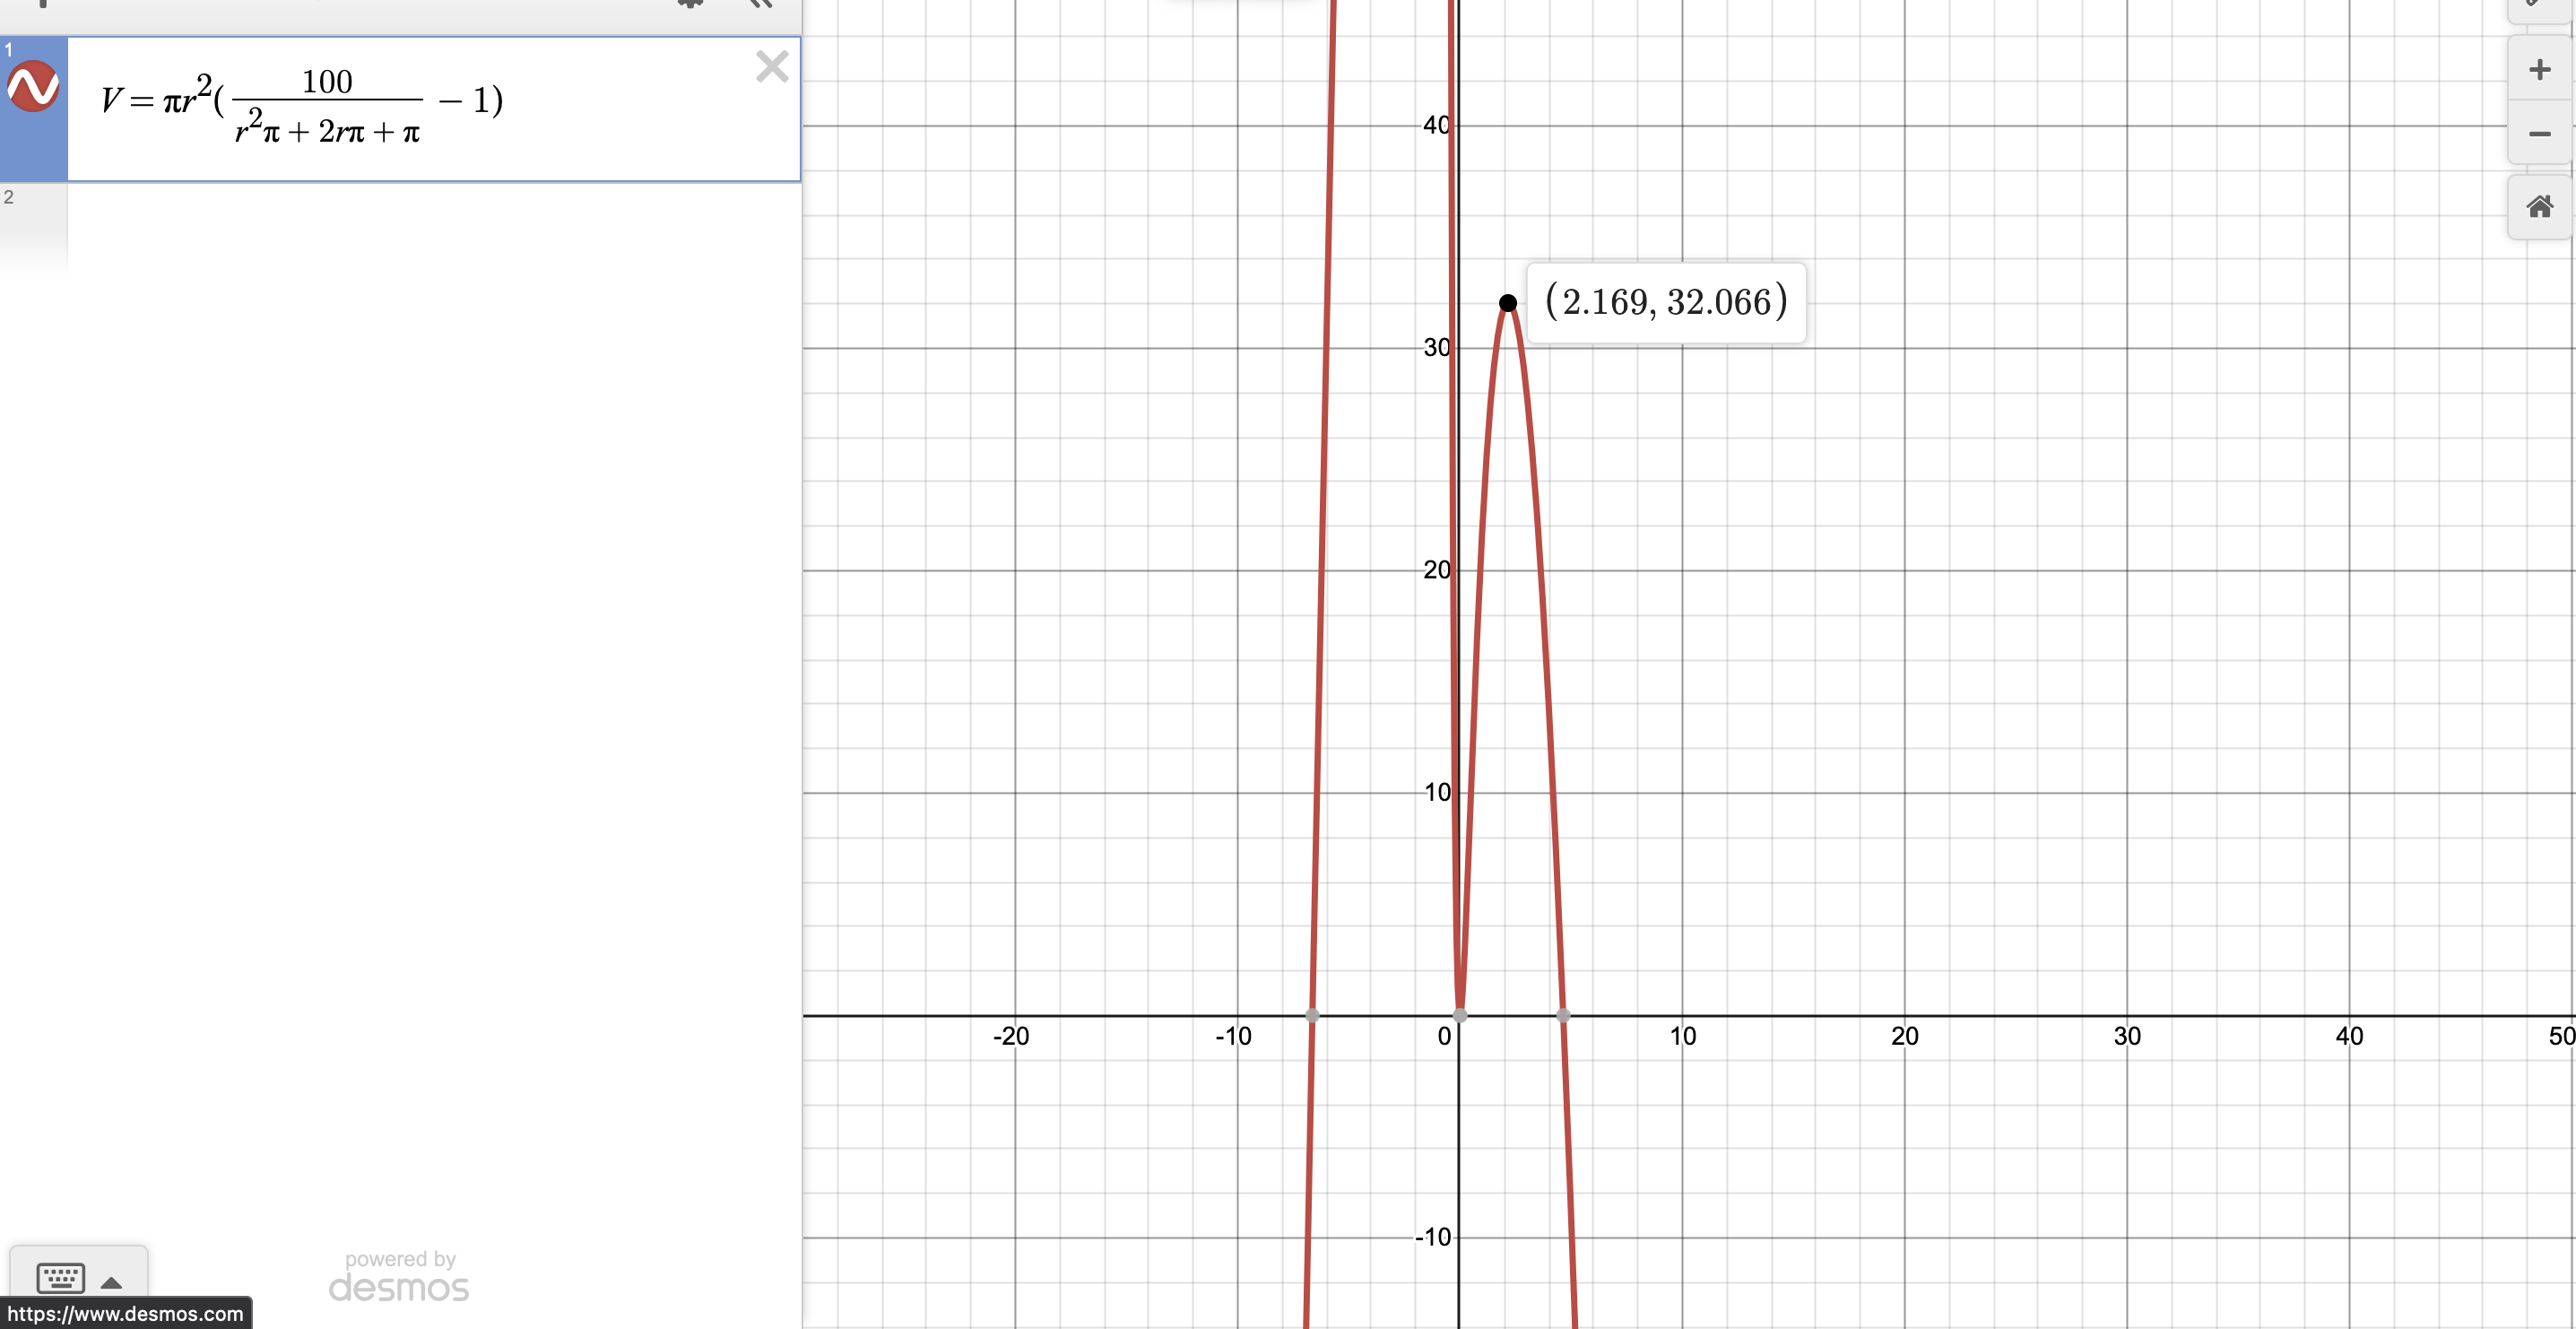
\includegraphics[width = 4in, height = 4in]{36}\newline 
From the graph, can see that the point $(2.169,32.066)$ is when the capacity is maximized. Points where $x\le 0$ do not make sense, as the radius must be a positive measurement. 
Thus the values for $r$ and $h$ that maximize the capacity of the tank are $2.169$ and
\[ \frac{100}{(2.169)^2\pi +2(2.169)\pi +\pi}-1\approx 2.1696 \] respectively.

\end{document}
